
\chapter{Introduction}

Time series is an important category of data since climate, finance, and health data all can be structured as time series. 
Classical regression, clustering and classification of time series data often works by analysing the observed values directly. 
Ordinal Patterns (OPs) take a different approach to time series analysis.
Instead of using the observed values, OPs transform those values into symbols.
These symbols retain information about the relative values, and aspire to capturing relevant information about the time series and the process that produced it.

Ordinal Patterns have been around for twenty years.
They were proposed by Bandt and Pompe in 2002~\cite{Bandt2002}.
This seminal article has received, to date, over \num{3000} citations on the Web of Science.
Their main properties are invariance, robustness, and being model-agnostic.

OPs have been used in applications in several domains.
Many of these applications involve comparing time series, signals, and images through features extracted from their Ordinal Patterns.
The ten most cited recent citations of Bandt and Pompe's paper deal with walnut crack detection~\cite{Zhang2024}, 
schizophrenia~\cite{Wang2024}, 
analysis of smart drilling~\cite{Szwajka2024}, 
epileptic seizure detection~\cite{AbhishekParikh2024}, 
mind wandering during video-based learning~\cite{Tang2024}, 
and random numbers generated based on dual-channel chaotic light~\cite{Liu2024}. 
%The rest that was found~\cite{Demirel2024, Du2024, Sun2024, Li2024}

We were interested in verifying the reproducibility of results of Ordinal Patterns in the scientific literature.

Initially, we wanted to check how many of those \num{3000} articles, were reproducible. 
This was a big task, so at first it was narrowed down to just papers focusing on climate. 
In the end, around \num{31} papers were investigated deeply.

Since results about the distribution of such features are recent, our initial interest was comparing existing conclusions with those supported by the new statistical tests.
While approaching this research avenue, we found indications of reproducibility crisis~\cite{Fidler2018} in this field, mostly related to data availability.
We then moved into the application of these new tests to already published results, and found evidence of the other type of reproducibility crisis: diverging results depending on the type of library employed.

Such a divergence stems from the definition of OPs.
The original proposal assigns a unique symbol to small subsets of the time series,
provided all the values are different.
If there are ties, the assignment is arbitrary.
Also, the technique does not stipulate how to handle missing (NA) values.

We decided to study the effect of preprocessing of the data by a combination of omitting NA values and adding noise to break ties. 
A new tie breaking method is proposed and its performance on computing entropy and $p$-values is investigated.

\chapter{Ordinal Patterns}

\section{History}
Bandt and Pompe's first paper about ordinal patterns is from 2002. 
They introduced the concept of turning a time series or signal into a sequence of symbols. 
They furthermore used the Shannon entropy on the symbol distribution~\cite{Bandt2002}. 
The Shannon Entropy was developed in 1948 by C.\ E.\ Shannon~\cite{Shannon1948} as a way to quantify uncertainty and unpredictability.

The 1995 paper ``A statistical measure of complexity'' by López-Ruiz et al.~\cite{LopezRuiz1995} introduced the concept of a statistical measure of complexity. 
This idea was applied to OPs in 2003~\cite{Martin2003}, and in 2004 the version of it using Jensen-Shannon divergence was published~\cite{Lamberti2004}.
We use the latter in this work.

\section{Definition}

Every analysis that employs OPs starts by defining the (integer-valued) word size $D\in\{2,3,\dots\}$ and time lag $\tau$.
We will only use $\tau=1$, and thus will drop it from the following discussion.

Consider the finite time series of real values $\bm x=(x_1, x_2,\dots, x_{n+D-1})$. 
The most common choices for the word size $D$, as seen in the bibliometric analysis below, are between three and six.
The Bandt \& Pompe transformation (also called ``BP Symbolisation'') converts each subset of size $D$ of contiguous and different values into a symbol, i.e.,
the first tuple of $D$ values will be $(x_1,x_2,\dots,x_{D})$, 
the second tuple will be $(x_2, x_3,\dots,x_{D+1})$, and so on.

There are at least two ways of computing OPs.
We will describe one of them.
Each tuple is transformed into a pattern by ranking the values. 
The lowest observation gets assigned the number $0$ and the highest observation gets the number $D-1$. 
The pattern can then be written as a string of these numbers. 
The tuple $(0.51, 0.79, 0.14)$ will have the pattern $1,2,0$.
How we write the patterns is transparent, provided there is only one pattern for each possible sorting of the tuple.
For example, we could have defined that $(0.51, 0.79, 0.14)$ becomes $\pi^3$ or $c$ or $\mathfrak{c}$.
Assuming there are no ties in each word, there are $D!$ possible patterns that we will denote $\bm\Pi=\{\pi^1,\pi^2,\dots,\pi^{D!}\}$.
Fig.~\ref{fig:ExampleProportions} shows an example of the observed proportions of OPs from a sequence of \num{1000} pseudorandom observations with $D=3$.

\begin{figure}[hbt]
	\centering
	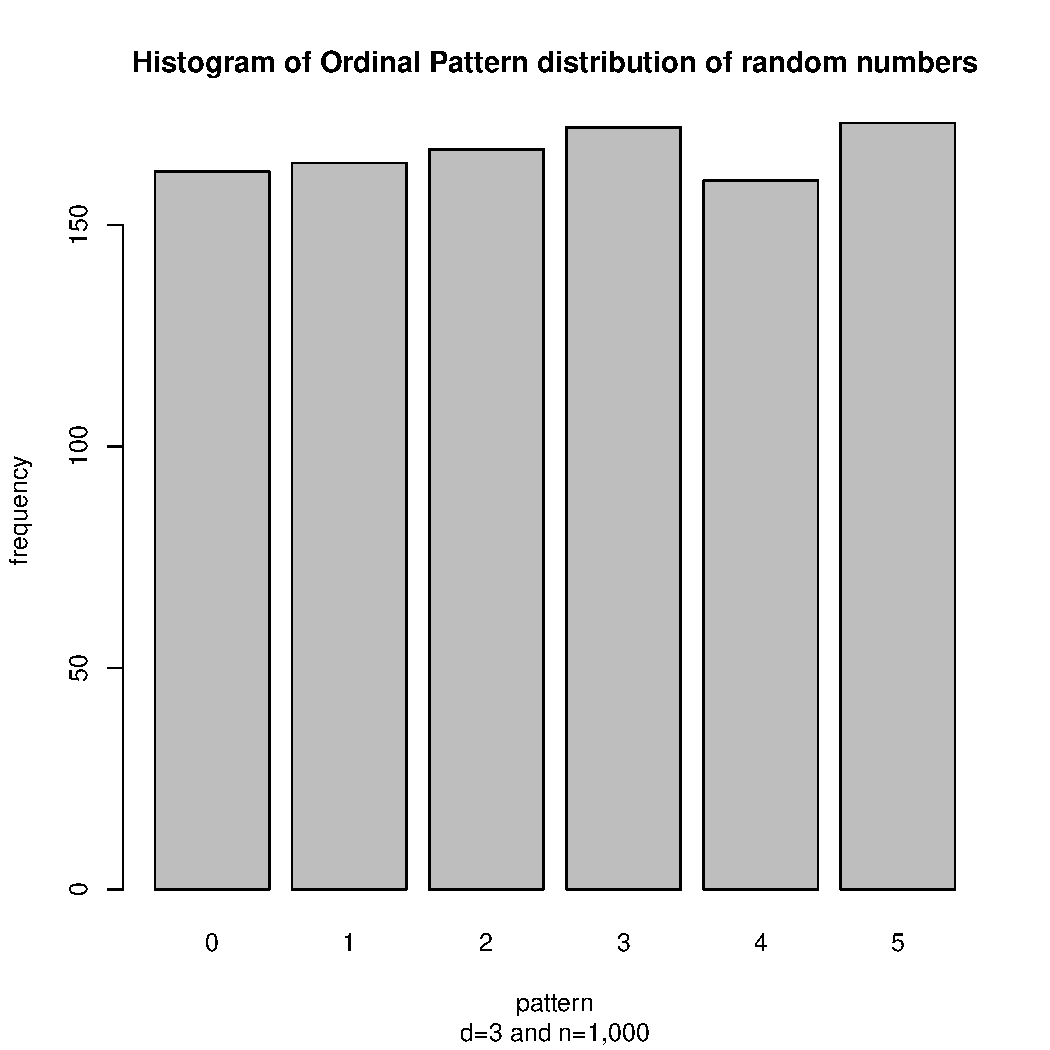
\includegraphics[width=.6\textwidth,keepaspectratio]{./powerlaw/histogram.pdf}
	\caption{Simple histogram of the ordinal pattern distribution of random numbers}
	\label{fig:ExampleProportions}
\end{figure}

By applying the BP symbolisation, we transform the time series 
$\bm x = (x_1, x_2, \dots, x_{n+D-1})$ into the sequence of symbols
$\bm \pi = (\pi_1, \pi_2,\dots, \pi_n)$.
The observed frequency of pattern $\pi^i$, denoted $\widehat{p}_i$, is defined as,
$$
\widehat{p}_i=\frac{\#\{t : \pi_t = \pi^i\}}{n} ,
$$
with which we define the vector of observed proportions:
$$
\widehat{\bm p} = (\widehat{p}_1, \widehat{p}_2, \dots, \widehat{p}_{D!}).
$$

A tie is when a tuple contains identical values. In practice, there may be ties, for instance when observing times series registered with finite precision.
There are several ways to handle ties.
They can be ignored, i.e., no pattern is computed for tuples with ties,
or they can be broken by adding small random perturbations. 
Techniques that handle ties are usually referred to as ``imputation solutions''~\cite{PermutationEntropyBasedTimeSeriesAnalysisEqualitiesintheInputSignalCanLeadtoFalseConclusions}.

OPs are usually considered useful for time series of at least length $n>100D$.

From the ordinal pattern distribution, features can be extracted. 
The two main used features in this field are Entropy and Complexity. 
In this paper, Shannon Entropy will be used, which is defined as.
$$
h(\widehat{\bm p})=-\sum_{i=1}^{D!} \widehat{p}_i \ln \widehat{p}_i,
$$
and its normalized version is:
$$
H(\widehat{\bm p})=-\frac{\sum_{i=1}^{D!} \widehat{p}_i  \ln \widehat{p}_i}{\ln D!}.
$$

There are several statistical complexity measures that can be used. 
They are all a product between the used entropy and a distance measure. 
Martin, Plastino and Rosso~\cite{Martin2003} used the Jensen-Shannon divergence between the pattern distribution and a reference distribution:
\begin{equation}
	Q'(\widehat{\bm p}, \bm{u}) = \sum_{i=1}^{D!} \Big(\widehat{p}_i \log\frac{\widehat{p}_i}{u_i} +
	u_i \log\frac{u_i}{\widehat{p}_i}
	\Big).
	\label{eq:JensenShannon}
\end{equation}
Most works consider the uniform distribution $\bm u = (1/D!, 1/D!, \dots, 1/D!)$ as the reference model, with which holds that
$$
\max\{Q'\} = -2\Big[
\frac{D!+1}{D!} \log(D!+1) - 2 \log(2D!) + \log D!
\Big],
$$
and we can define the normalized Jensen-Shannon distance as $Q(\widehat{\bm p}, \bm{u})=Q'(\widehat{\bm p}, \bm{u})/\max\{Q'\}$.

With this, Lamberti et al.~\cite{Lamberti2004} proposed $C(\widehat{\bm p})=H(\widehat{\bm p})Q(\widehat{\bm p}, \bm{u})$ as a measure of the Statistical Complexity of the underlying dynamics.
Notice that both $H(\widehat{\bm p})$ and $Q(\widehat{\bm p}, \bm{u})$ are normalized quantities, so also is $C(\widehat{\bm p}, \bm{u})$. 

Not all values in $[0,1]^2$ are possible
Martin et al.~\cite{GeneralizedStatisticalComplexityMeasuresGeometricalandAnalyticalProperties}, using geometrical arguments on the space of configurations, found expressions for the boundaries of the feasible values.
The lower boundary $C_{\min}$ is smooth, while the upper $C_{\max}$ is defined by $D!-1$ pieces.
The upper boundary converges to a smooth curve when $D\to\infty$.
The set of possible values is called ``Entropy-Complexity'' or ``$H\times C$ plane,'' although it is not a plane but a closed set embedded in $[0,1]^2$.

Quoting Ref.~\cite{WhiteNoiseTestfromOrdinalPatternsintheEntropyComplexityPlane}:
\begin{quote}
Fig.~\ref{fig:Boundaries} shows the boundaries of the $H\times C$ plane for the embedding dimensions $D=3$ (red) $D=4$ (green), and $D=5$ (blue).
The inset plot highlights the fine structure of the upper boundary inside the rectangle.
The jagged structure of $C_{\max}$ increases the difficulty of finding distributions for the points in the $H\times C$ plane.
\end{quote}

\begin{figure}[hbt]
	\centering
	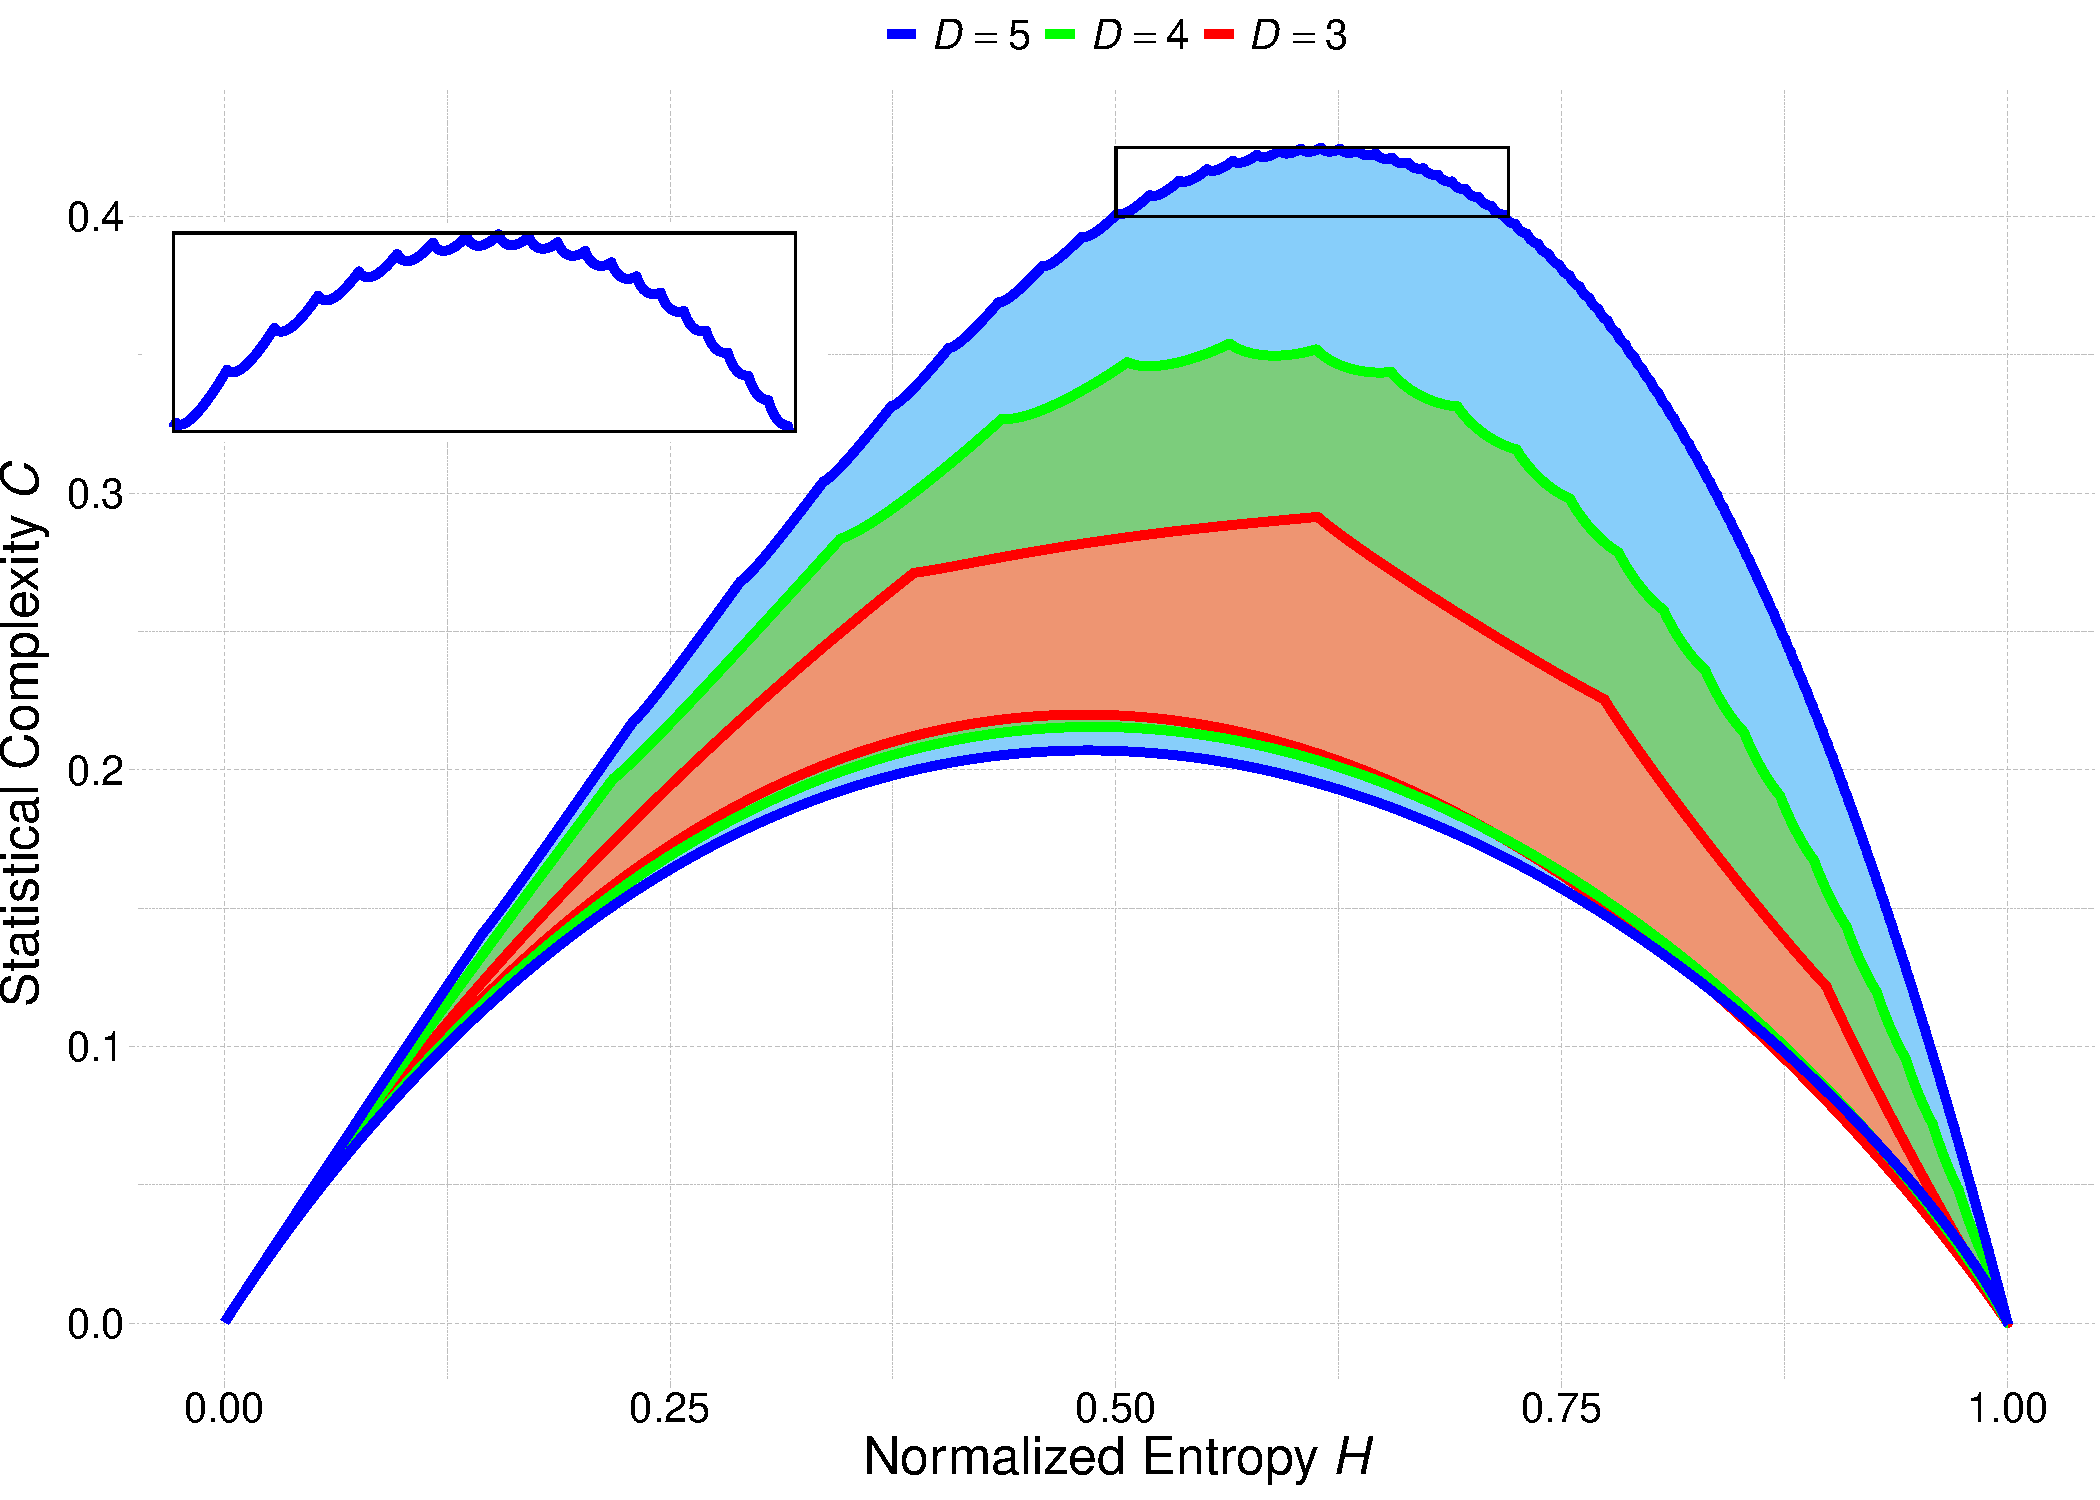
\includegraphics[width=.7\linewidth]{../../Figures/BoundariesPlot}
	\caption{Boundaries of the $H\times C$ plane for dimension embeddings $D=3,4,5$. From: Chagas et al.~\cite{WhiteNoiseTestfromOrdinalPatternsintheEntropyComplexityPlane}}\label{fig:Boundaries}
\end{figure}

\section{Reproducibility}

Data from many scientific fields are analysed in data science, as shown in the application section of ordinal patterns above. 
It therefore increases the difficulty of reproducing the data collection stage, as most cases require an interdisciplinary study involving multiple people. 
In some cases, it is impossible, e.g., if the equipment needed is unavailable or a time series of weather data cannot be recollected, since it is impossible to go back in time. 
The point of science is to eliminate trust when sharing knowledge, however, the above observations highlight the need for some degree of confidence, in cases, where data cannot be reproduced. 

The COVID-19 pandemic gave birth to the following quote. 
``We warn against the potential misuse or misleading interpretation of public data of variable quality''~\cite{Struelens2021}. 
Data from different governments do not have the same quality. 
This necessitates good source criticism.
 
In this paper, data from peer-reviewed studies will be trusted, which have often either produced the data themselves or got it from reputable organizations such as NASA or NOAA. 
Only pseudorandom numbers, that is, generated by a script on a reproducible computer environment, will be produced in this paper.

In this paper, the focus will be on direct computational reproduction.
We quote Fidler and Cox~\cite{Fidler2018} as a guide for our study:
\begin{quote}
``Computational reproducibility is most often direct (reproducing particular analysis outcomes from the same data set using the same code and software), but it can also be conceptual (analysing the same raw data set with alternative approaches, different models or statistical frameworks).''
\end{quote}


\section{Bibliometric analysis}

Ideally, all papers should be reproducible and especially their data processing part, since modern technology allows for extremely efficient data sharing across vast distance to a very affordable price. 
According to Baker~\cite{Baker2016}, more than \SI{70}{\percent} of researches have failed reproducing an article and \SI{52}{\percent} agree that there is significant reproducibility crisis. 

We observed cases where the data had been downloaded and verified to being true, but the data processing could not be reproduced.
The article by Saco et al.~\cite{Saco2010} is an example.
Figures~\ref{fig:OriginalEntropy} shows a plot from that work.
We downloaded the data the authors reported, and obtained Fig.~\ref{fig:ReplicatedStudy}.
The discrepancy is obvious.
We contacted the corresponding author, but have not received a response.

\begin{figure}[hbt]
	\centering
	\subcaptionbox{Reported entropy values; red dots should be as in Fig.~\ref{fig:ReplicatedStudy}\label{fig:OriginalEntropy}}
	{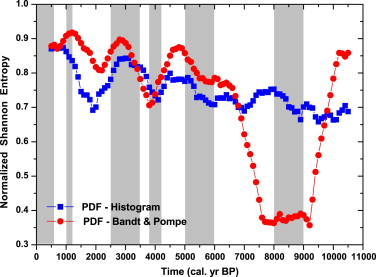
\includegraphics[width=.48\textwidth,keepaspectratio]{ElNino/ArticleEntropyPlot.jpg}}
	\subcaptionbox{Replicated data.\label{fig:ReplicatedStudy}}
	{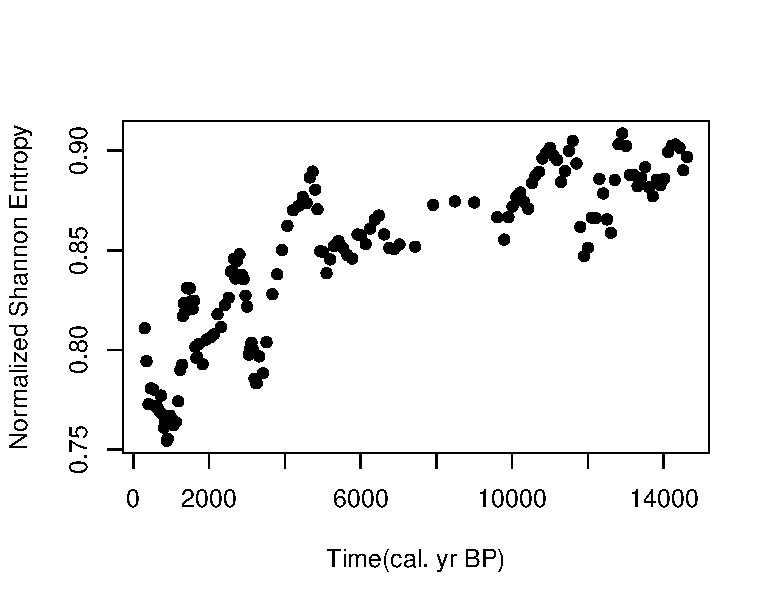
\includegraphics[width=.48\textwidth,keepaspectratio]{ElNino/Entropy.pdf}}
	\caption{Diverging results}\label{fig:Diverging}
\end{figure}

We analysed \num{31} articles for data availability and used word size ($D$). 
The majority of them are about climate, and they explicit have to used Permutation Entropy. Four categories were made for data availability: “Available”, “Sourced”, “On-Request” and “Not Available”. 

Sourced~(S) is the broadest category. 
Some articles give a detailed description of how to pull the data from a website. 
Other articles give no description, except which organisation they got the data from. 
The is no differentiation between these cases in the category S. 
Available~(A) is the best category and only used when the data is directly downloadable. 
On Request~(R) is when the dataset has to be requested by the author and is suboptimal. 
Not Available~(N) is the worst category, because there is no source to data, nor is the dataset attached to the paper in any way. 

Only four articles had data readily downloadable. 
The data is definitely possible to get from some articles in category "S", but many of them were very sparse in their description of the data, to the point where it was be hard to pull it from the website. 
Assuming that around half of the data from articles in ``S'' can be pulled from their sources, that leaves around \SI{50}{\percent} of the articles for which it is not possible to reproduce the data processing part. 
Table~\ref{tab:ArticlesPerData} summarises these findings.

\begin{table}[hbt]
	\centering
	\begin{tabular}{*4{c}}
		\toprule
		A & S  & R & N \\ \midrule
		4 & 19 & 3 & 4 \\ \bottomrule
	\end{tabular}
	\caption{Number of articles per data availability.}\label{tab:ArticlesPerData}
\end{table}

Word sizes between two and seven were used. 
Some articles used multiple word sizes, which is why the sum of ``No. articles using'' is higher than \num{31}.
Table~\ref{tab:ArticlesPerD} for the aggregated values.

\begin{table}[hbt]
\centering
\begin{tabular}{*8{c}}
\toprule
Word size $D$ & 2 & 3  & 4  & 5 & 6 & 7 & Multiple \\ \midrule
No. articles using  & 4 & 13 & 15 & 9 & 6 & 1 & 9        \\ \bottomrule
\end{tabular}
\caption{Number of articles per word size ($D$) used.}\label{tab:ArticlesPerD}
\end{table}


